%%% LaTeX Template
%%% This template is made for project reports
%%%	You may adjust it to your own needs/purposes
%%%
%%% Copyright: http://www.howtotex.com/
%%% Date: March 2011

%%% Preamble
\documentclass[paper=a4, fontsize=11pt]{scrartcl}	% Article class of KOMA-script with 11pt font and a4 format
\usepackage[T1]{fontenc}
\usepackage{fourier}

\usepackage[english]{babel}															% English language/hyphenation
\usepackage[protrusion=true,expansion=true]{microtype}				% Better typography
\usepackage{amsmath,amsfonts,amsthm}										% Math packages
\usepackage[pdftex]{graphicx}														% Enable pdflatex
\usepackage{url}
\usepackage{graphicx}
\usepackage{hyperref}

%%% Custom sectioning (sectsty package)
\usepackage{sectsty}												% Custom sectioning (see below)
\allsectionsfont{\centering \normalfont\scshape}	% Change font of al section commands


%%% Custom headers/footers (fancyhdr package)
\usepackage{fancyhdr}
\pagestyle{fancyplain}
\fancyhead{}														% No page header
\fancyfoot[C]{}													% Empty
\fancyfoot[R]{\thepage}									% Pagenumbering
\renewcommand{\headrulewidth}{0pt}			% Remove header underlines
\renewcommand{\footrulewidth}{0pt}				% Remove footer underlines
\setlength{\headheight}{13.6pt}


%%% Equation and float numbering
\numberwithin{equation}{section}		% Equationnumbering: section.eq#
\numberwithin{figure}{section}			% Figurenumbering: section.fig#
\numberwithin{table}{section}				% Tablenumbering: section.tab#


%%% Maketitle metadata
\newcommand{\horrule}[1]{\rule{\linewidth}{#1}} 	% Horizontal rule

\title{
		%\vspace{-1in} 	
		\usefont{OT1}{bch}{b}{n}
		\normalfont \normalsize \textsc{University of Chicago Dept of Genetic Medicine} \\ [25pt]
		\horrule{0.5pt} \\[0.4cm]
		\huge PGRNseq Analysis \\
		\horrule{2pt} \\[0.5cm]
}
\author{
		\normalfont 								\normalsize
        Vassily Trubetskoy \\[-3pt]		\normalsize
        \today
}
\date{}


%%% Begin document
\begin{document}
\maketitle

\section{Overview}

Notes on the on going analysis of genetic data in patients undergoing treament with Irinotecan. The current iteration of the study contains data from samples collected across three different sites. In all, there are currently 253 individuals with targeted sequence and Illumina exome chip data. Samples were collected from patients undergoing a chemotherapeutic regimen with Irinotecan.

\newpage

\section{Data}

	\subsection{Genotypes}

We currently have access to two different sets of genotypes for this population:
	
	\begin{enumerate}
		\item PGRNseq sequence data on VIP pharmacogenes.
		\item Illumina Exome Chip data. Run as an internal QC measure at the UW.
	\end{enumerate}
	
We have the alignment files for the sequence data. These were run through the consensus calling pipeline on Amazon.

	\subsection{Phenotypes}
	
The primary phenotype for this dataset is pharmacokinetic and pharmacodynamic data on patients. These PK/PD models are being generated at the University of North Carolina Chapel Hill.

In addition to PK/PD phenotypes, we are interested in looking at Neutropenia in patients. This is currently coded as the Neutrophil Count Nadir (NCN). This is defined as the lowest Neutrophil count observed in a patient during their course of therapy.

There are several relevant covariates available:
	\begin{itemize}
		\item site of collection
		\item sex
		\item drug dose
		\item self-reported ancestry
	\end{itemize}

	\subsection{Quality Control}
	Consensus calling in the sequence data. The results look very nice for the metrics that we have available (reference separate report, or put figures here).
	
	\begin{itemize}
		\item Exclude rare SNPs in single marker analyses
		\item Exclude SNPs out of HWE (has not yet been done)
		\item Exclude SNPs with high rates of genotype missingness
		\item Exclude SNPs with low QUAL
		\item Check PGRNseq and Exome chip genotype concordance
	\end{itemize}

	\subsubsection{Genotype Concordance}
	Checking concordance between PGRNseq and Exome chip genotypes. \\
	
	Number of overlapping variant sites: 883 \\
	Number of non-overlapping variant sites: 7850 \\
	Genotype concordance: 0.9494 \\
	
	This seems low, but the vast majority of sites contain perfectly concordant calls. The average is significantly lowered due to ~30 sites with near-zero concordance. 
	
	\subsection{Proposed Analyses}
	\begin{itemize}
		\item Linear regression. Using the estimated effect and its eror as a t-statistic. (GenABEL package in R)
		\item SKAT burden test. (SKAT package in R)
	\end{itemize}
	
\newpage

\section{Results}

	\subsection{Population Structure}
Sequence data provides too few variants to adequately identify ancestry through PCA .

The Exome chip data \emph{does} provide enough markers to differentiate samples. The spatial axes are well defined (see \hyperref[exomeAncestry]{Fig 3.1}). These PC's were used to identify a set of genetically homogenous samples (see \hyperref[exomeCluster]{Fig 3.2} and \hyperref[exomeCEUZoom]{Fig 3.3}).

%%% FIGURES
\begin{figure}[exomeAncestry]
\centering
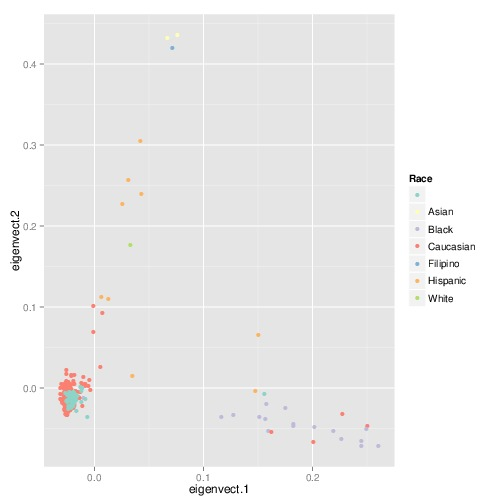
\includegraphics[scale=1.0]{{{plots/exomeChip.PCA.selfReportedAncestry}}}
\caption{First two principal components of exome chip genotype data. The samples segregate fairly well into their self-reported ancestries.	}
\end{figure}

\begin{figure}[exomeCluster]
\centering
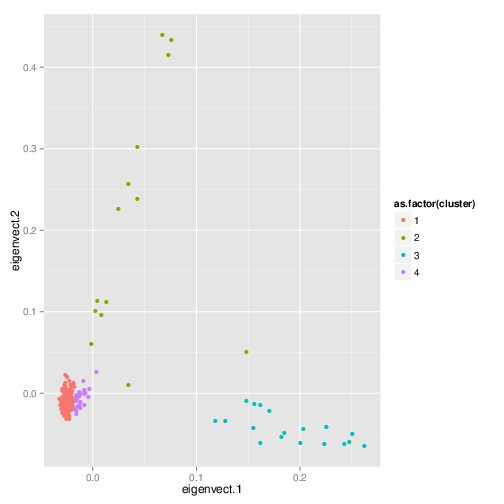
\includegraphics[scale=1.0]{{{plots/exomeChip.PCA.clustering}}}
\caption{Model based clustering of the first two pricipal components using the exome chip genotypes. These clusters were used to select a homogenous set of samples. In this case, we subset our data to the 161 samples contained in cluster 1.}
\end{figure}

\begin{figure}[exomeCEUZoom]
\centering
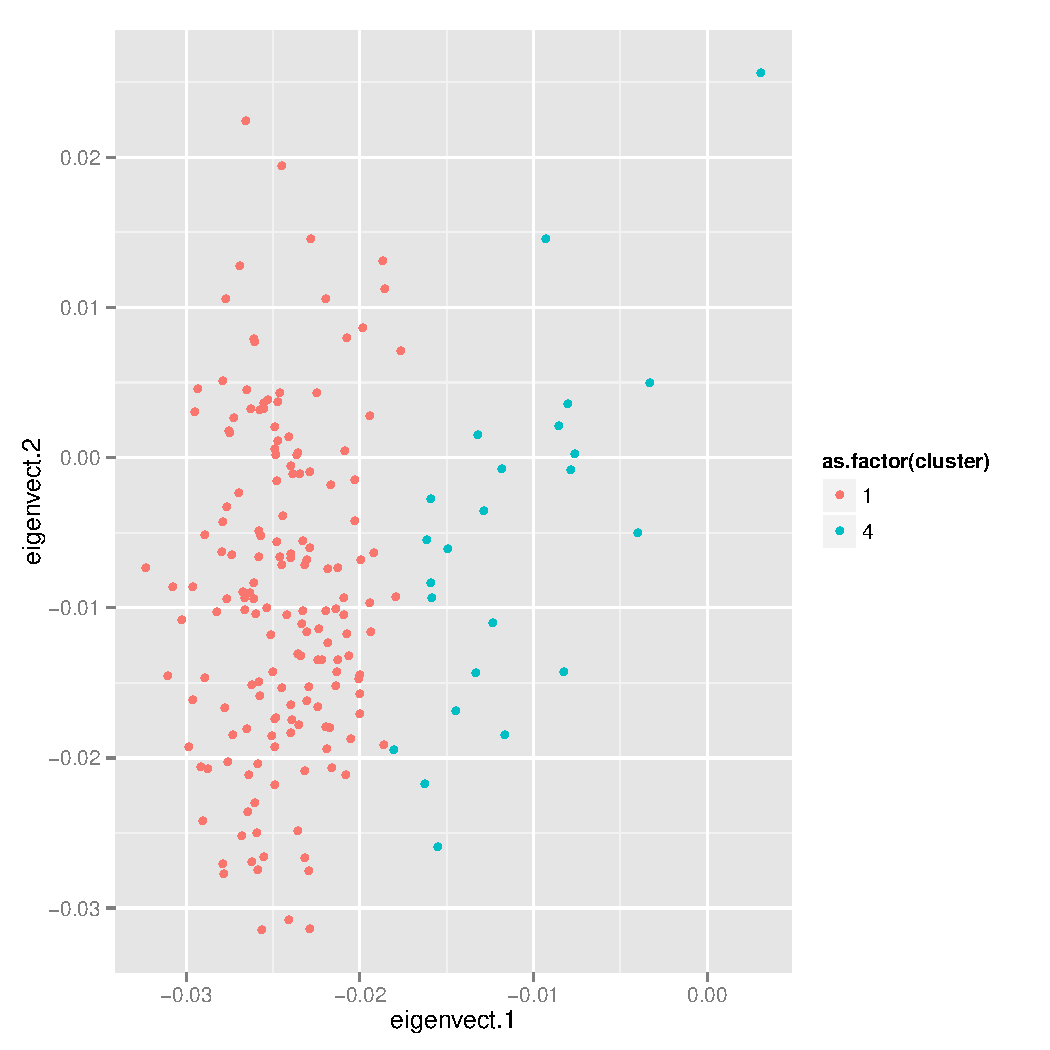
\includegraphics[scale=1.0]{{{plots/exomeChip.PCA.clustering.CEUzoom}}}
\caption{A zoom of the European cluster in the exome chip PCA. This shows some substructure, and we ultimately subset the samples contained in cluster 1.}
\end{figure}

	\subsection{Single Marker}
		\subsubsection{Notes and Issues}
		There may be some genomic inflation present in the single marker tests. This needs to be formally reported as a calculation of lambda.	
	
		\subsubsection{GenABEL Linear Regression}
		No results in sequence data for common variants. The QQ plot without covariates shows some deflation in the tail (see \hyperref[basicSeqQQ]{Fig 3.4}). Once adjusting with available covarites, the scan looks reasonably null (see \hyperref[fullSeqQQ]{Fig 3.5}). \\
		
		One significant marker in Exome chip data, with a couple of suggestive hits. The p-value improves with a full model including covariates. \\
		
\begin{table}
\begin{center}
\begin{tabular}{ccccccc}
var ID & p-val & chr & loc & UCSC gene \\ \hline
exm899253 & 1.611e-06 & 11 & 33596398 & KIAA1549L \\ \hline
exm1065858 & 2.292e-06 & 13 & 42390907 & VWA8 \\ \hline
exm1362200 & 8.388e-06 & 17 & 77078092 & ENGASE\\ \hline
exm1453164 & 1.120e-05 & 19 & 33579109 & GPATCH1 \\ \hline
\end{tabular}
\caption{Top four results for the single marker exome scan. These correspond to the QQ plot found in \hyperref[fullExomeQQ]{Fig 3.7}}
\label{exomeRegRes}
\end{center}
\end{table}
		
		\begin{figure}[basicSeqQQ]
		\centering
		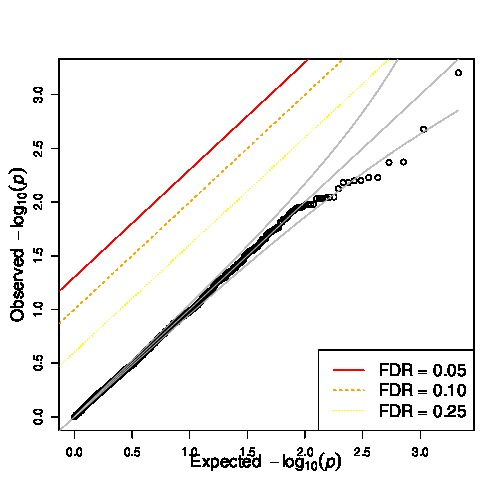
\includegraphics[scale=1]{{{plots/sequence.gwa.basicmodel.qq}}}
		\caption{GWA scan for sequence data using the basic model: $ANC = Geno$. SNPs were excluded based on the following criteria: call rate $<0.95$, MAF $<0.05$, and HWE. Individuals were excluded based on missing phenotype and PCA outliers. This result was produced with 160 individuals with 2,140 markers. There is some deflation seen in extremely small p-values.}
		\end{figure}	
		
		\begin{figure}[fullSeqQQ]
		\centering
		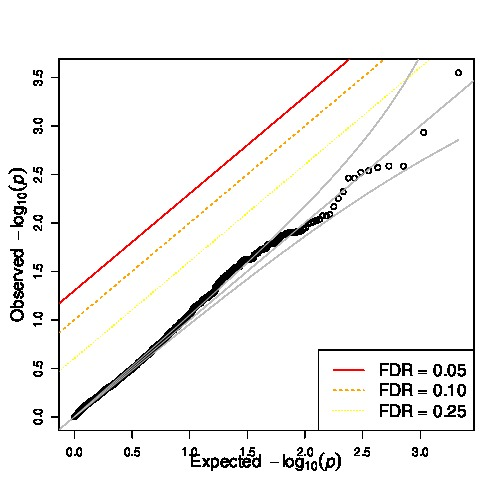
\includegraphics[scale=1]{{{plots/sequence.gwa.fullmodel.qq}}}
		\caption{GWA scan for sequence data using the full covariate model: $ANC = Geno + sex + site + dose$. SNPs were excluded based on the following criteria: call rate $<0.95$, MAF $<0.05$, and HWE. Individuals were excluded based on missing phenotype and PCA outliers. This result was produced with 160 individuals with 2,140 markers. The covariate correction reduces the deflation observed at small p-values.}
		\end{figure}			
		
		\begin{figure}[basicExomeQQ]
		\centering
		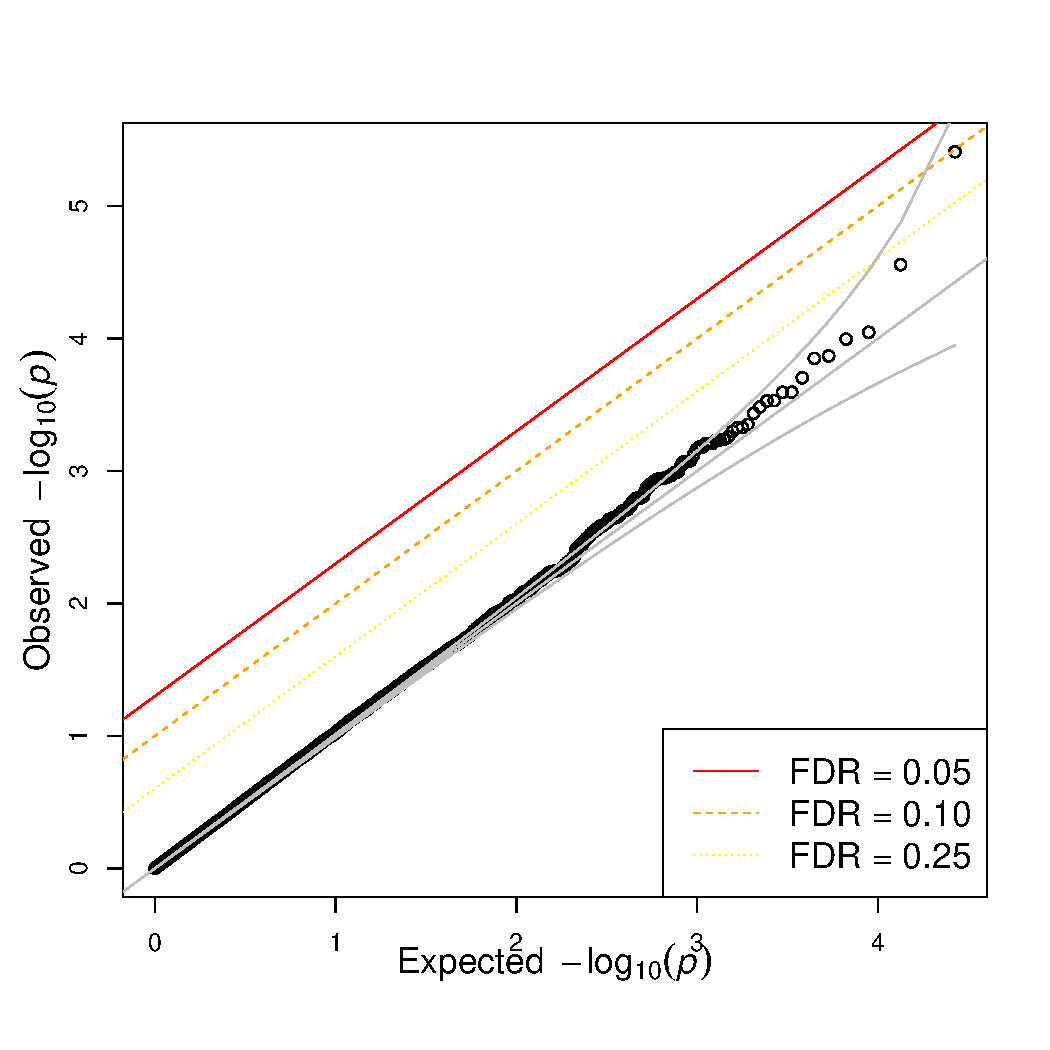
\includegraphics[scale=1]{{{plots/exome.gwa.basicmodel.qq}}}
		\caption{GWA scan for exome chip data using the basic model: $ANC = Geno$. SNPs were excluded based on the following criteria: call rate $<0.95$, MAF $<0.05$, and HWE. Individuals were excluded based on missing phenotype, missing covariate and PCA outliers. The final dataset consisted of 159 individuals and 26,728 markers.}
		\end{figure}	
		
		\begin{figure}[fullExomeQQ]
		\centering
		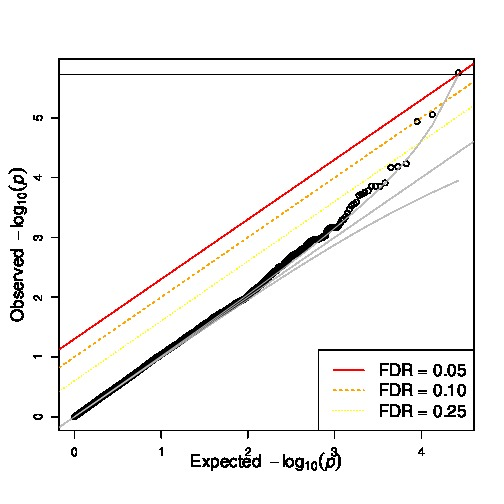
\includegraphics[scale=1]{{{plots/exome.gwa.fullmodel.qq}}}
		\caption{GWA scan for exome chip data using the full covariate model: $ANC = Geno + sex + site + dose$. SNPs were excluded based on the following criteria: call rate $<0.95$, MAF $<0.05$, and HWE. Individuals were excluded based on missing phenotype, missing covariate and PCA outliers. The final dataset consisted of 159 individuals and 26,728 markers.}		
		\end{figure}
		
	\subsection{Gene-based}
		\subsubsection{Notes and Issues}
		I'll have to think some more about which SKAT test is appropriate for this data. There is an excellent article by Lee et. al (2012) that proposes the optimal rare variant test SKAT-O. This statistic is a linear combination of burden and variance component statistics. You can also specify different kernels. The default kernel weights variants based on rareness.
		
		The variants need to be cleaned. Right now, a lot of genes are dropped due to high rates of missingness. Additionally, many genotypes are being imputed through the SKAT package based on HWE.
		
		I am not using the finite sample correction that the author's suggest for $n<2000$. P-values are computed with a parametric bootstrap with $n=10000$ iterations.		
		
		\subsubsection{SKAT Burden}
		Currently running for the model: $ANC = Geno + sex + site + dose$. Eleven samples are excluded for having missing covariate information. Many sites contain high rates of missingess, and imputation is performed by the SKAT package. \hyperref[SKATburdenQQ]{Fig 3.4} shows the QQ-plot that contains a number of significant associations in the tail. These top hits are summarized in the \hyperref[burdenResults]{Table 3.1}.

\begin{table}
\begin{center}
\begin{tabular}{cccccc}
ENTREZ ID & SKAT asymptotic p & Num. Snps & Symbol \\ \hline
3177 & 8.183411e-08 & 8 & SLC29A2 \\ \hline
6799 & 2.130900e-05 & 14 & SULT1A2 \\ \hline
8824 & 3.287893e-04 & 78 & CES2 \\ \hline
6817 & 5.014952e-02 & 27 & SULT1A1 \\ \hline
4881 & 6.311036e-04 & 27 & NPR1 \\ \hline
\end{tabular}
\caption{Top five results for the burden test. P-values were generated with an theoretical distribution of the test, as well as with $10^{5}$ bootstrap iterations in a resampling procedure. The expensive nature of bootstrap means that the smallest possible observable pvalue is $10^{-5}$.}
\label{burdenResults}
\end{center}
\end{table}

\begin{figure}[SKATburdenQQ]
\centering
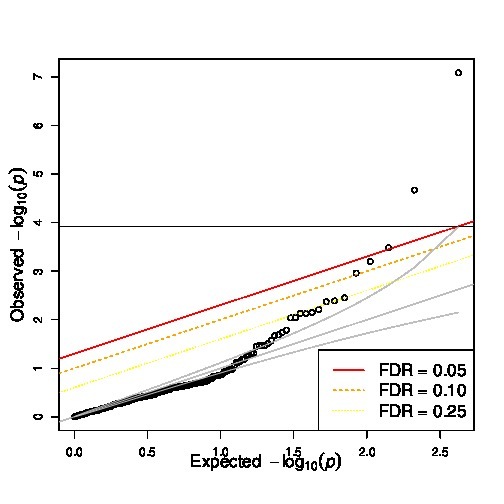
\includegraphics[scale=1.0]{{{plots/SKAT.burdenQQ}}}
\caption{QQ plot from a set of 421 gene-based units tested with SKAT's burden test in 150 individuals. P-values were generated with a theoretical distribution (though the top hit is maintained with a resampling based p-value). }
\end{figure}	

		\subsubsection{SKAT Rare + Common}
		Many of the variants are rare in this dataset. Our top hits are nearly identical to the burden top hits since the common test is being down weighted.


\section{References}


%%% End document
\end{document}
